\documentclass[a4paper,10pt]{article}
\usepackage[lmargin=2.0cm, rmargin=1.0cm,tmargin=3.5cm,bmargin=1.5cm]{geometry}
\usepackage{color,graphics}
\usepackage[export]{adjustbox}
\usepackage{lipsum}
\usepackage{comment}
\usepackage{graphicx}
\usepackage{grffile}
\usepackage{hyperref}
\usepackage{listings}
\usepackage[scaled=0.75]{helvet}
\usepackage{listings}
\usepackage{color}
\usepackage[final]{pdfpages}
\definecolor{dkgreen}{rgb}{0,0.6,0}
\definecolor{gray}{rgb}{0.5,0.5,0.5}
\definecolor{mauve}{rgb}{0.58,0,0.82}

\lstset{frame=tb,
	language=Java,
	aboveskip=3mm,
	belowskip=3mm,
	showstringspaces=false,
	columns=flexible,
	basicstyle={\small\ttfamily},
	numbers=none,
	numberstyle=\tiny\color{gray},
	keywordstyle=\color{blue},
	commentstyle=\color{dkgreen},
	stringstyle=\color{mauve},
	breaklines=true,
	breakatwhitespace=true,
	tabsize=3
}

\begin{document}
\setcounter{secnumdepth}{-1} 

\begin{center}
\textbf{\LARGE Installation and Working On Multi Node Hadoop Cluster.}
\end{center}

\raggedright Expt No: 4 \hfill \raggedleft March  20, 2019 \\ 

\raggedright Author: Subalakshmi Shanthosi S  (186001008) \par 

\noindent\makebox[\linewidth]{\rule{\textwidth}{1pt}} 

\section{Aim}
Installation of Hadoop in multi node cluster.

\section{Software's Used}
\begin{itemize}
	\item Ubuntu  16.04 LTS
	\item Hadoop 1.0.3
\end{itemize}

\section{Description}
\begin{enumerate}
	\item A Multi Node cluster in Hadoop comprises of Two or More DataNodes.
	\item A hadoop cluster can be referred to as a computational computer cluster for storing and analysing big data (structured, semi-structured and unstructured) in a distributed environment.
	\item Components of Hadoop HDFS:
	\begin{enumerate}
		\item Master Node – 
		\begin{itemize}
			
		\item Master node in a hadoop cluster is responsible for storing data in HDFS and executing parallel computation the stored data using MapReduce.
		\item Master Node has 3 nodes :
		\begin{itemize} 
			\item NameNode
			\item Secondary NameNode 
			\item JobTracker
		\end{itemize} 
		\item JobTracker monitors the parallel processing of data using MapReduce.
		\item NameNode handles the data storage function with HDFS. \item The secondary NameNode keeps a backup of the NameNode data.
	\end{itemize}
	\item 	Slave/Worker Node- 
	\begin{itemize}
		\item This component in a hadoop cluster is responsible for storing the data and performing computations. 
		\item Every slave/worker node runs both a TaskTracker and a DataNode service to communicate with the Master node in the cluster. 
		\item The DataNode service is secondary to the NameNode and the TaskTracker service is secondary to the JobTracker.
	\end{itemize}
	\item Client Nodes - 
	\begin{itemize}
		\item Client node has hadoop installed with all the required cluster configuration settings and is responsible for loading all the data into the hadoop cluster. 
		\item Client node submits mapreduce jobs describing on how data needs to be processed and then the output is retrieved by the client node once the job processing is completed.
	\end{itemize}
	\item Differences between Single Node and MultiNode clusters:
	\begin{itemize}
		\item Hadoop installed on multi node cluster is more efficient.
		\item In the single node cluster, all the necessary demons like NameNode, DataNode, Resource Manager, Node manager and Application master etc run on the same machine but different ports.
		\item Multi node cluster follows Master-Slave architecture. In multi node cluster (distributed mode), they run on different machines (master and slave).
		\item The replication factor for multi node cluster will be more than one and it should be installed in more than one machine to satisfy the Master-Slave architecture.
		\item Multi node cluster is basically used for full stack development of hadoop application and projects whereas Single Node Cluster is for testing purpose
	\end{itemize}
	\pagebreak
	\item Components of Multi Node Cluster and Architecture: 
	 \begin{figure}[h]
	 	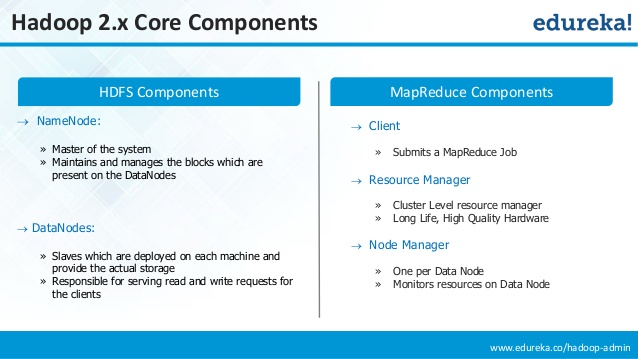
\includegraphics[scale=0.45,center]{exptFourScreenShot/HadoopMultiNodeComponents.jpg}
	 	\caption{Hadoop Multi Node cluster components.}
	 	\label{fig:0.0.1}
	 \end{figure}

	 
	 \begin{figure}[h]
	 	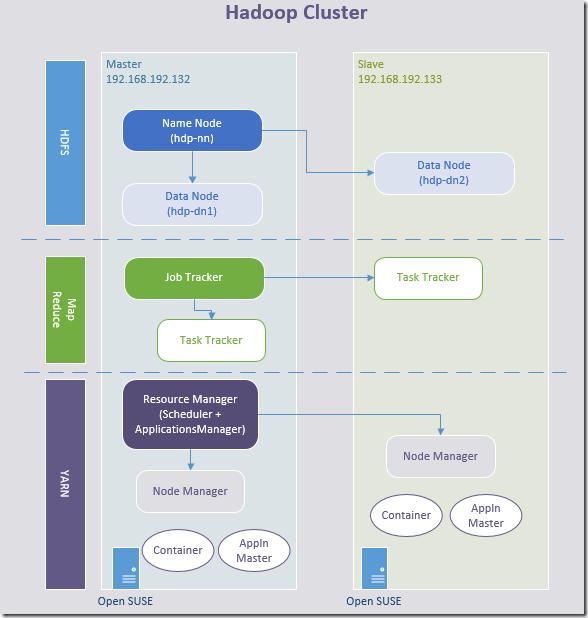
\includegraphics[scale=0.45,center]{exptFourScreenShot/HadoopMultiNode.png}
	 	\caption{Hadoop Multi Node cluster architecture.}
	 	\label{fig:0.0.2}
	 \end{figure}
	\end{enumerate}
\end{enumerate}

\section{Procedure - Steps Involved:}
\begin{itemize}
\item Configuring two Single node clusters by performing the following steps as follows.	
\begin{enumerate}
	\item Launch Ubuntu 16.04 LTS.
	\item Login to the OS with sudo permission and install the following packages using apt-get command.
	\begin{itemize}
		\item openssh-server
		\item openssh-client
		\item java jdk 8
		\item javac compiler
		\item hadoop 1.0.3
	\end{itemize}
	\item Create a new user with sudo permission (hduser:hadoop).
	\item Log into the hduser and do the following:
	\begin{itemize}
		\item Copy the hadoop executable to /usr/local directory.
		\item Install and configure appropriate environment variables and parameters in the following configuration files: 
		\begin{itemize}
			\item conf/hadoop-env.sh : Configure JAVA\_HOME and HADOOP\_HOME with appropriate values.
			\item conf/core-site.xml : Configure hadoop default temp directory and default file system.
			\item conf/mapred-site.xml : JobTracker name and port number.
			\item conf/hdfs-site.xml : Default replication factor specification.
		\end{itemize}
		\item Format the namenode by specified dfs.name.dir by running command : /usr/local/hadoop/bin/hadoop namenode -format .
		\item Starting the local hadoop single node cluster by running command: 
		/usr/local/hadoop/bin/start-all.sh .
		\item To check the current running Hadoop Processes by running command : 
		jps .
		\item Stopping the local hadoop single node cluster by running command : 
		/usr/local/hadoop/bin/stop-all.sh .
	\end{itemize}
 \item Networking:
 \begin{itemize}
 	\item Update /etc/hosts file with configuration as follows in both the machines:
 	\begin{figure}[h]
 		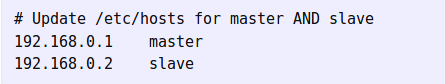
\includegraphics[scale=0.45,center]{exptFourScreenShot/NetConfInNodes.png}
 		\caption{Networking configuration in Master and Slave nodes.}
 		\label{fig:0.1}
 	\end{figure}
 \end{itemize}	
 \pagebreak
 \item Configuring SSH Access:
 \begin{itemize}
   \item Adding hduser{\fontfamily{ptm}\selectfont @}master public SSH key to the authorized\_keys file of hduser{\fontfamily{ptm}\selectfont @} slave .
   \begin{figure}[h]
   	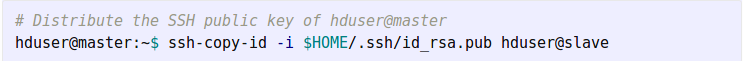
\includegraphics[scale=0.45,center]{exptFourScreenShot/sshAccess.png}
   	\caption{Copying SSH public key to slave from master node.}
   	\label{fig:0.2}
   \end{figure}
   \begin{figure}[h]
   	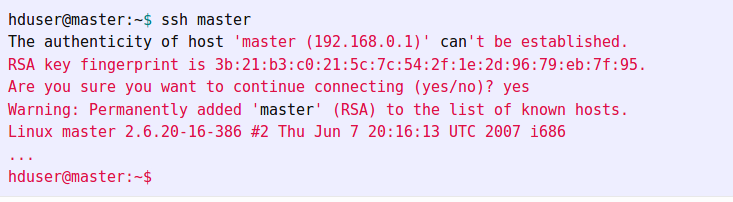
\includegraphics[scale=0.45,center]{exptFourScreenShot/sshMaster.png}
   	\caption{SSH to master node.}
   	\label{fig:0.3}
   \end{figure}
   	\begin{figure}[h]
   		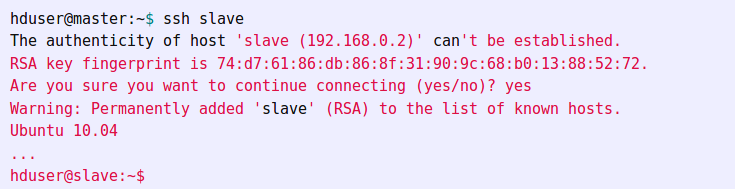
\includegraphics[scale=0.45,center]{exptFourScreenShot/sshSlave.png}
   		\caption{SSH to Slave node.}
   		\label{fig:0.4}
   	\end{figure}
 \end{itemize}
\end{enumerate}
\end{itemize}



		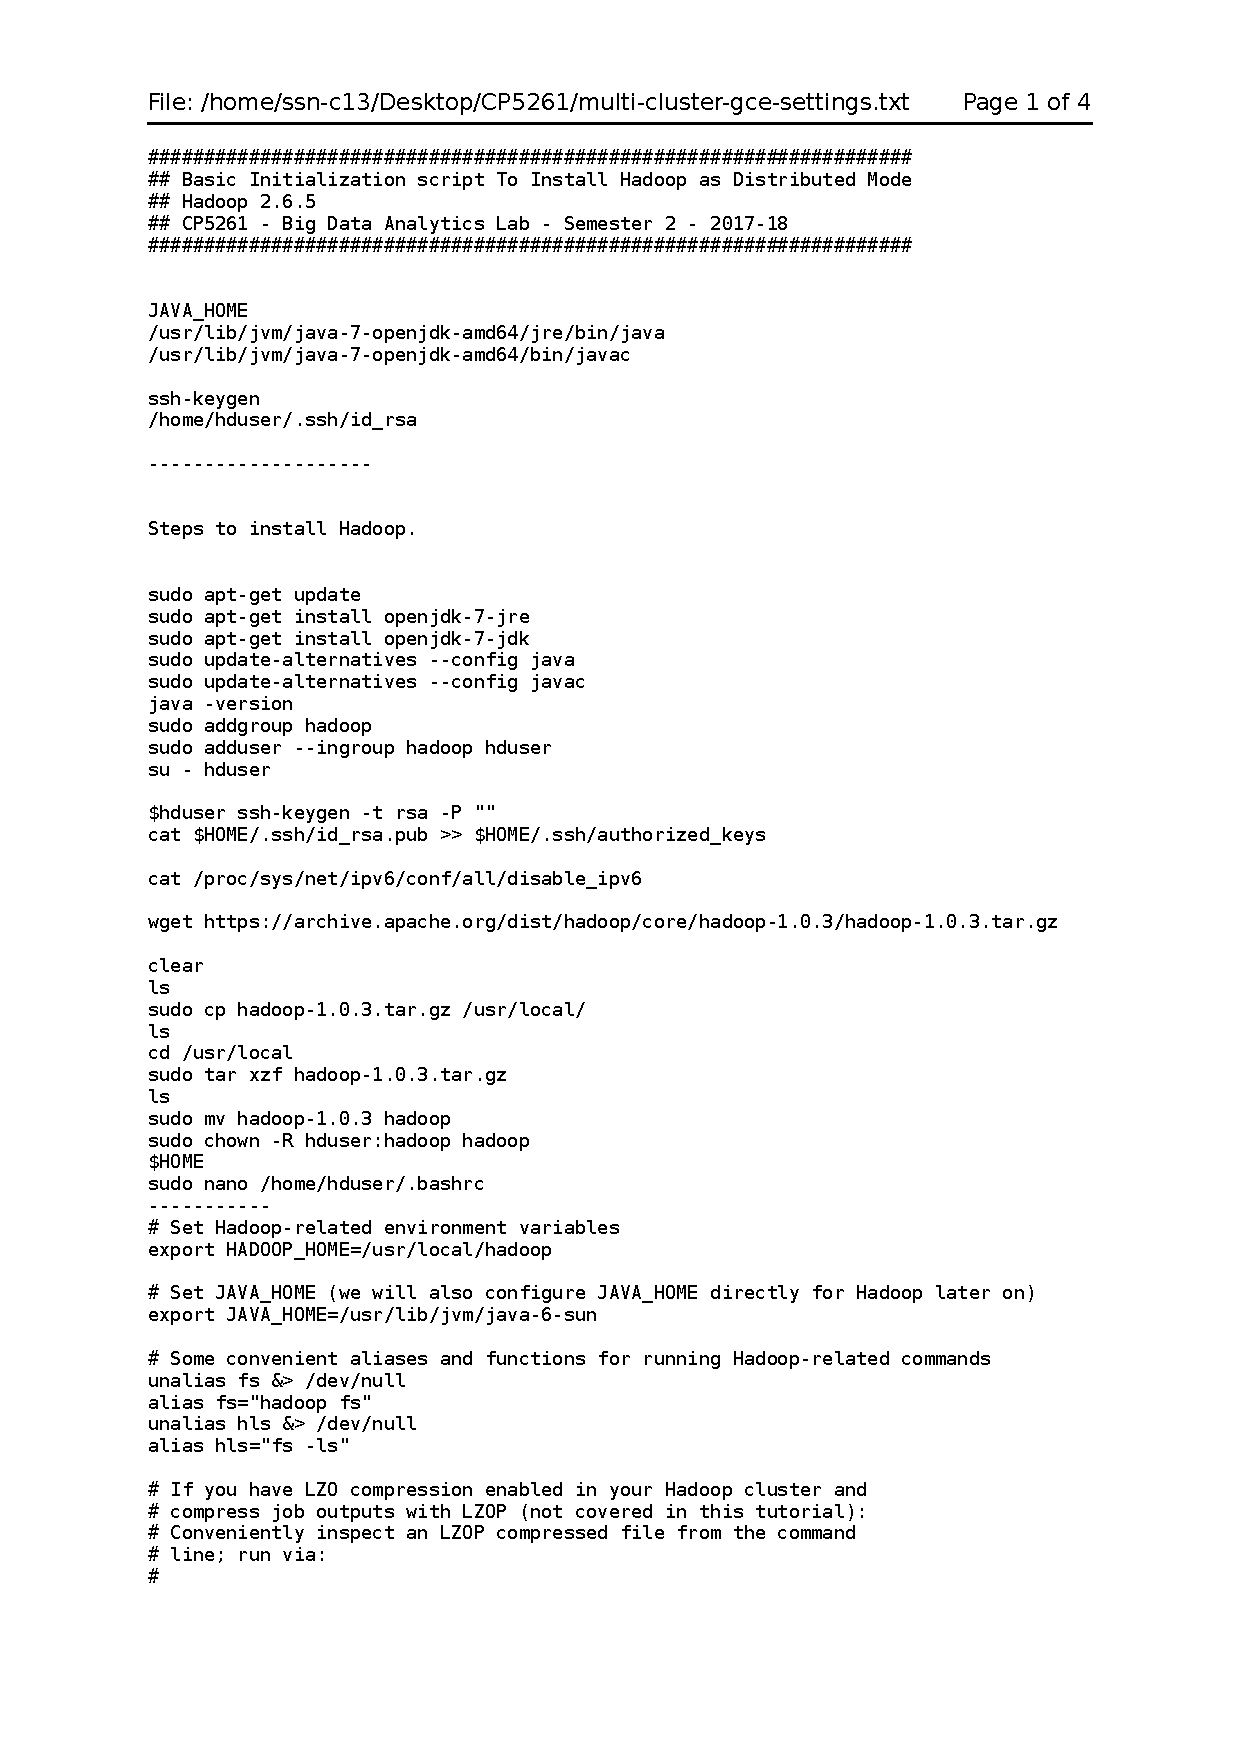
\includepdf[pages=1,pagecommand={},noautoscale = true,scale=1.03]{Ex-4-hadoop-installation-multi.pdf}
		\includepdf[pages=2,pagecommand={},noautoscale = true,scale=1.03 ]{Ex-4-hadoop-installation-multi.pdf}
		\includepdf[pages=3,pagecommand={},noautoscale = true,scale=1.03 ]{Ex-4-hadoop-installation-multi.pdf}
		\includepdf[pages=4,pagecommand={},noautoscale = true,scale=1.03]{Ex-4-hadoop-installation-multi.pdf}

\end{document}
